\chapter{Design Principles for Energy--Efficient Applications}

%Use IEEE Software article plus some from "What Got Us Here" and expand both, then answer RQ.

\section{Introduction}

Digital-transformation initiatives have led to major efficiencies and cost savings, including the transition from paper-based processing to electronic documents and the use of traffic-routing algorithms for vehicle navigation. However, the software performing this remarkable work consumes nearly 10 percent of the world's electricity \cite{mills2013-digital-energyusage}. Today's cloud-based applications span multiple continents, consuming energy in servers, networks, cooling and power facilities, storage, and user devices.

In this chapter we present three simple design principles software architects can use to address system-level energy efficiency. A case study illustrates the energy savings possible with a holistic approach.

Over the past decade, researchers have been studying IT infrastructure energy consumption, working to increase datacenter, network, and hardware efficiency. Datacenter energy efficiency has improved considerably. For example, in the US, public-sector datacenters are now expected to operate at a power usage effectiveness (PUE) of less than 1.5, whereas a PUE of 2 was considered normal only a few years ago.

PUE is a datacenter's total energy consumption divided by its IT energy consumption, usually measured over one year. A PUE of 1.5 indicates that for every 1 KWh of IT load, a datacenter requires an additional 0.5 KWh.
Hardware has experienced a similar trend; computations per joule of energy have doubled every 1.57 years over the past two decades \cite{koomey2011-trends-energy-efficiency}. Yet, limited progress has been made in addressing the entire software system's energy efficiency. However, software engineering research is now focusing on a system-wide approach.

\section{The Challenge for Software Architects}

We suspected that software architects might find it difficult to prioritize energy efficiency for three main reasons. 

First, we have little understanding of how design decisions affect energy efficiency or other system qualities such as user experience, reliability, and performance. Without this knowledge, analyzing tradeoffs to elucidate the benefits or costs of improving energy efficiency is difficult. Minor system design changes could yield substantial benefits, such as avoiding unnecessary polling or eliminating redundant housekeeping tasks that prevent equipment from entering lower power states. However, a lack of relevant design tools and frameworks makes it difficult for architects to achieve more sophisticated optimizations that consider contextual information about the runtime environment.

Second, to achieve the next order of magnitude in energy efficiency, architects must think beyond traditional design boundaries. This will require that people from different specializations and departments work together. Such collaboration is challenging given current organizational software governance structures, wherein teams might have competing objectives, and human dynamics and political barriers. Moreover, existing technologies provide few mechanisms to allow communication across different technology layers (the application software, middleware, hardware, network, cooling, power infrastructure, and so on), which would enable cross-layer optimization.

Finally, end users rarely require or worry about energy efficiency. On one hand are split incentives. System operators such as administrators or datacenter managers don’t pick up the energy bill—the money tends to come out of the facilities budget. Accordingly, they would see little return from any energy savings. On the other hand, given current energy prices, information and communications technology energy costs constitute less than 3 percent of a typical organization’s budget. So, when an organization pursues energy efficiency, it often does so by addressing areas with a larger budget share (such as payroll!) Exacerbating this problem is the lack of benchmarks, metrics, and reliable data that would allow realistic comparisons of different energy efficiency opportunities and their returns.

\textbf{TODO} - reference the "What Software Architects Think" section from the Data Centre Energy Demand chapter.  See if I can write more about that.

\section{State of the Art}

To increase efficiency, we must be able to measure it. That is, we must be able to measure the useful work our software applications produce and the amount of energy this takes and then optimize the ratio between the two. However, although the datacenter world has metrics such as PUE, no comparable metrics exist for software.

A further complication is that modern applications run across multiple platforms (user devices, networks, computers, storage, and so on). Optimizing energy consumption across all these platforms will require a range of specialists to collaborate across traditional design boundaries.

Optimization must also consider key quality properties such as resilience (because redundancy in system designs is usually a major contributor to energy consumption), usability, and performance. In reality, however, we have no design tradeoff tools that let us conduct such analyses \cite{bashroush2016-datacentreenergy}.

Despite these challenges, energy efficiency has been gaining traction in software engineering. Much of the early research focused on measuring applications' energy consumption \cite{islam2016-energysoftwarefeatures} and tried to define useful work so as to allow the creation of useful metrics (for example, the DC4Cities project; www.dc4cities.eu). In parallel, other researchers have explored compiler optimization to decrease energy consumption or have evaluated design patterns' energy efficiency.

All these efforts have helped us begin to understand and optimize software applications. However, improving today's Internet-scale systems will require a more radical approach that considers the whole system. Such an approach is inherent to software architecture work.

\section{The Three Principles}

On the basis of early experiences and research in the field, we propose three simple architecture principles for achieving energy-efficient systems:

\begin{itemize}
\item \emph{Principle 1}. Energy efficiency metrics must relate business transactions to energy consumption in a meaningful way to key system stakeholders.
\item \emph{Principle 2}. Identifying sources of energy waste at the system level produces the biggest savings.
\item \emph{Principle 3}. Addressing the energy optimization problem requires a cross-disciplinary team.
\end{itemize}

We now examine these principles in more detail.

\textbf{TODO} these can be expanded significantly

\subsection{Relating Business Transactions to Energy Consumption}

Energy efficiency must be measured in a way that system stakeholders can understand. Ensuring that the metrics are meaningful is necessary to convince senior management to sponsor optimization projects. Ultimately, suitable metrics can help achieve holistic system tuning and drive revenue and cost optimization.

\subsection{Identifying Sources of Waste}

Focus effort where it will be the most effective. For example, redundancy is a commonly overlooked source of energy consumption. To support resilience, redundancy is usually applied at all levels, including facilities, hardware, and software. Without system-level evaluation of resilience requirements, redundancy might be applied too generously. So, matching redundancy to actual requirements is a huge opportunity to achieve energy savings that would be difficult with local optimizations.

\subsection{Employing Cross-Disciplinary Teams}

Energy optimization requires design work across traditional design boundaries. For example, optimizing the design of resilience requires collaboration among infrastructure engineering, application development, and business teams. Without such collective efforts, improvements will be restricted to local optimizations, which often miss the bigger opportunities for savings.

\section{Case Study: Online Auction Site}

The online-auction company eBay used principles such as those we have outlined to achieve significant energy savings.

As part of eBay's commitment to reducing its environmental footprint while decreasing costs and increasing performance, it introduced the Digital Service Efficiency (DSE) initiative \cite{ebay2013-digitalefficiency}. DSE relates business metrics such as customer buying and selling transactions to their energy consumption and environmental impact. DSE provides a set of easily understood metrics to help eBay understand, communicate, balance, and tune its energy consumption (principle 1). These metrics include: Buy Transactions / kWh; Sell Transactions / kWh; Revenue / MW; and CO2 emissions / Million users to name a few.

eBay identified reducing infrastructure redundancy as one of the main opportunities to save energy. To explore this opportunity, eBay rethought its entire system architecture (principle 2), taking into consideration its business needs and redundancy costs. eBay realized that no matter how resilient its back-end system was, if the end-user system failed, the whole session failed. This meant that responsibility for system resilience could be moved to the weakest link: the end-user system.

So, the company introduced a new system architecture that includes a monitor in the end-user system. The monitor identifies when a transaction such as a search request exceeds a timeout, perhaps owing to a service failure. When this occurs, the monitor transparently reissues the request to another service location, without notifying the user. Thus, noncritical services can be less resilient because the monitor's operation can mask their failures.

Furthermore, on the basis of business analytics, eBay estimated that only about 10 percent of its transactions were critical, such as payments. Payment handling has specific regulatory needs and requires a highly available infrastructure. On the basis of this insight, eBay processes payments at a specific, highly resilient datacenter that's a fraction of the capacity of its original datacenter \emph{[Dean Nelson's talk "How eBay's I and O Organization Is Supporting Business Initiatives" from Gartner Data Center Conf. 2013] - not available?} while processing the remaining workload in a cheaper, less resilient infrastructure. This significant improvement in energy efficiency required cooperation across eBay's engineering, operational, and business teams (principle 3).

Figure \ref{figure:styles} depicts eBay's original and resulting architectures. The new design allows for reduced datacenter redundancy while maintaining overall system performance and resilience.

\begin{figure}
\centering
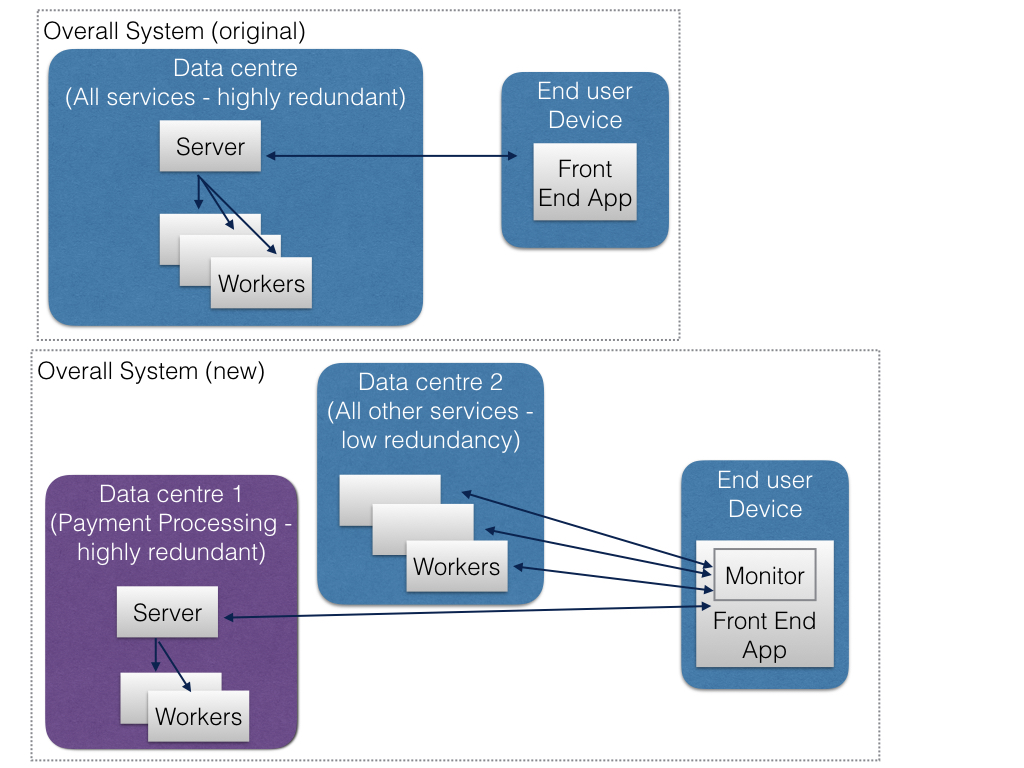
\includegraphics[width=\textwidth]{Figures/principles-styles}
\caption{eBay's (a) original system architecture and (b) new design}
\label{figure:styles}
\end{figure}

eBay has achieved major capital and operational expenditure savings by adopting this new architecture. The new low-redundancy site's simpler requirements have substantially decreased the infrastructure, which in turn has significantly decreased datacenter build-out and fit-out costs and time scales. Redundancy costs are significant. For example, according to Steven Shapiro, the cost of building a Tier III datacenter is double that of a Tier II datacenter \cite{shapiro2015-datacentre-mythsrealities}. (The Tier Classification System is a widely used rating system for datacenter availability, with Tier I being the least available or redundant facility and Tier IV the highest \cite{uptime2015-tierclassification}.)

Even more important (from our perspective), eBay has reduced energy consumption by approximately 50 percent because the low-redundancy site requires fewer infrastructure components (for example, N + 1 rather than 2N + 1 redundancy).5 This has resulted in not only significant energy cost savings but also reduced maintenance and hardware refresh requirements, further lowering environmental costs.

\section{Conclusion}

There has been increased interest in reducing the significant energy costs of running large IT systems. However, software architects lack suitable tools and methods to address energy concerns when designing systems. With this challenge in mind, we've suggested our three principles, which architects can follow to make energy-related tradeoffs during system design even with today's limited knowledge and technology.

Despite these principles' simplicity, eBay's experience shows that they can yield significant cost and energy savings when applied to large-scale production systems. Savings of this scale are difficult to achieve through local optimizations, so we must rely on software architects' skills to lead our efforts in this emerging area




